\section{Floquet Fermi Goldern Rule}

In this section we are going to derive the Floquet Fermi goldern rule for above derived quantum Floquet states using $t-t'$ formalism.

\vspace{5mm}
\noindent
The Floquet states \eqref{3.17} fullfills the $t-t'$ Schrödinger equation [*Ref:myReport] as follows
\begin{equation} \label{4.1}
  i \hbar \pdv{t}\ket{\psi_{\alpha}(t,t')} =
  H_F(t') \ket{\psi_{\alpha}(t,t')}
\end{equation}
where Floquet Hamiltonian given by
\begin{equation} \label{4.2}
  H_F(t') \equiv
  H_e(t) - i\hbar \dv{t}
\end{equation}
and
\begin{equation} \label{4.3}
  \ket{\psi_{\alpha}(t,t')} =
  \exp(-\frac{i}{\hbar}\varepsilon_{\alpha} t)\ket{\phi_{\alpha}(t')}
\end{equation}
Now for the Eq. \eqref{4.1} corresponding time evolution operator satisfy the Schrödinger equation
\begin{equation} \label{4.4}
  U_0(t,t_0;t') = \exp(-\frac{i}{\hbar}H_F(t')\qty[t-t_0])
\end{equation}
Consider a time-independent total perturbation $V(\mb{r})$ switched on at the reference time $t-=t_0$, then Schrödinger equation becomes
\begin{equation} \label{4.5}
  i \hbar \pdv{t}\ket{\Psi_{\alpha}(t,t')} =
  \qty[H_F(t') + V(\mb{r})]\ket{\Psi_{\alpha}(t,t')}
\end{equation}
and when $t\leq t_0$ both solutions of the Schrödinger equation coincide
\begin{equation} \label{4.6}
  \ket{\psi_{\alpha}(t,t')} =\ket{\Psi_{\alpha}(t,t')} \quad
  \text{when} \quad
  t \leq t_0
\end{equation}
Now, we can introduce the interaction picture representation of the $t-t'$ Floquet state as
\begin{equation} \label{4.7}
  \ket{\Psi_{\alpha}(t,t')}_I = U_0^{\dagger}(t,t_0;t')
  \ket{\Psi_{\alpha}(t,t')}
\end{equation}
and the perturbation in the interaction picture will be
\begin{equation} \label{4.8}
  V_I(\mb{r}) = U_0^{\dagger}(t,t_0;t')V(\mb{r})U_0(t,t_0;t') =
  V(\mb{r}).
\end{equation}
This leads to the Schrödinger  eqution in the interction picture
\begin{equation} \label{4.9}
  i \hbar \pdv{t}\ket{\Psi_{\alpha}(t,t')}_I =
  V_I(\mb{r})\ket{\Psi_{\alpha}(t,t')}_I
\end{equation}
with the recursive solution
\begin{equation} \label{4.10}
  \ket{\Psi_{\alpha}(t,t')}_I = \ket{\Psi_{\alpha}(t_0,t')}_I +
  \frac{1}{i\hbar}
  \int_{t_0}^t dt_1 \;
  V_I(\mb{r}) \ket{\Psi_{\alpha}(t_1,t')}_I
\end{equation}
Iterating the solution only upto first order (Born approximation) this leads to
\begin{equation} \label{4.11}
  \ket{\Psi_{\alpha}(t,t')}_I \approx \ket{\psi_{\alpha}(t_0,t')} +
  \frac{1}{i\hbar}
  \int_{t_0}^t dt_1 \;
  V_I(\mb{r}) \ket{\psi_{\alpha}(t_0,t')}
\end{equation}
and multiply it by $\bra{\psi_{\beta}(t_0,t')}$ and we will get
\begin{equation} \label{4.12}
  \braket{\psi_{\beta}(t_0,t')}{\Psi_{\alpha}(t,t')}_I = \braket{\psi_{\beta}(t_0,t')}{\psi_{\alpha}(t_0,t')} +
  \frac{1}{i\hbar}
  \int_{t_0}^t dt_1 \;
  \bra{\psi_{\beta}(t_0,t')}
  V_I(\mb{r}) \ket{\psi_{\alpha}(t_0,t')}.
\end{equation}
Then introdusing unitory operator $U_0$ we can re-write this as
\begin{equation} \label{4.13}
  \begin{aligned}
    \mel{\psi_{\beta}(t_0,t')}{U_0^{\dagger}(t,t_0;t')}{\Psi_{\alpha}(t,t')} & = \mel{\psi_{\beta}(t_0,t')}{U_0^{\dagger}(t,t_0;t')U_0(t,t_0;t')}{\psi_{\alpha}(t_0,t')} \\
    & +
    \frac{1}{i\hbar}
    \int_{t_0}^t dt_1 \;
    \bra{\psi_{\beta}(t_0,t')}
    U_0^{\dagger}(t_1,t_0;t')
    V(\mb{r})
    U_0(t_1,t_0;t')
    \ket{\psi_{\alpha}(t_0,t')}
  \end{aligned}
\end{equation}
and this can be simplied as
\begin{equation} \label{4.14}
  \begin{aligned}
    \braket{\psi_{\beta}(t,t')}{\Psi_{\alpha}(t,t')} = \braket{\psi_{\beta}(t,t')}{\psi_{\alpha}(t,t')} +
    \frac{1}{i\hbar}
    \int_{t_0}^t dt_1 \;
    \bra{\psi_{\beta}(t_1,t')}
    V(\mb{r}) \ket{\psi_{\alpha}(t_1,t')}.
  \end{aligned}
\end{equation}
Since our $t-t'$ Floquet states are orthonormal [*Ref:myReport- t-t' formalism] we can derive that
\begin{equation} \label{4.15}
  \begin{aligned}
    \braket{\psi_{\beta}(t,t')}{\Psi_{\alpha}(t,t')} =
    \delta_{\alpha\beta}\exp(i\omega\qty[t'-t]) +
    \frac{1}{i\hbar}
    \int_{t_0}^t dt_1 \;
    \bra{\psi_{\beta}(t_1,t')}
    V(\mb{r}) \ket{\psi_{\alpha}(t_1,t')}.
  \end{aligned}
\end{equation}
Now, set $t_0 = 0$ and for a case $\alpha \neq \beta$ this will simplied to
\begin{equation} \label{4.16}
  \begin{aligned}
    \braket{\psi_{\beta}(t,t')}{\Psi_{\alpha}(t,t')} =
    -
    \frac{i}{\hbar}
    \int_{0}^t dt_1 \;
    \bra{\psi_{\beta}(t_1,t')}
    V(\mb{r}) \ket{\psi_{\alpha}(t_1,t')}.
  \end{aligned}
\end{equation}
In addition, since our Floquet states create a basis for composite space we can represent any solution using our Floquet states
\begin{equation} \label{4.17}
  \ket{\Psi_{\alpha}(t,t')} = \sum_{\beta} a_{\alpha\beta}(t,t')
  \ket{\psi_{\beta}(t,t')}.
\end{equation}
Therefore we can derive a equation for this \textit{scattering amplitude} as
\begin{equation} \label{4.18}
  a_{\alpha\beta}(t,t') =
  \braket{\psi_{\beta}(t,t')}{\Psi_{\alpha}(t,t')} =
  -
  \frac{i}{\hbar}
  \int_{0}^t dt_1 \;
  \bra{\psi_{\beta}(t_1,t')}
  V(\mb{r}) \ket{\psi_{\alpha}(t_1,t')}.
\end{equation}

\vspace{5mm}
\noindent
Now lets assume a scattering event from a $t-t'$ Floquet state $\ket{\psi_{\beta}(t,t')}$ into another $t-t'$ Floquet state $\ket{\Psi_{\alpha}(t,t')}$ with constant quansienergy $\varepsilon$ given as follows
\begin{equation} \label{4.19}
  \ket{\Psi_{\alpha}(t,t')} =
  \exp(-\frac{i}{\hbar}\varepsilon t)
  \ket{\Phi_{\alpha}(t')}
\end{equation}
Now consider a scattering event
\begin{equation} \label{4.20}
  \psi_{\beta}(\mb{k'},t,t') = \exp(-\frac{i}{\hbar}\varepsilon_{\beta} t)
  \phi_{\beta}(\mb{k'},t')
  \longrightarrow
  \Psi_{\alpha}(\mb{k},t,t') = \exp(-\frac{i}{\hbar}\varepsilon t)
  \Phi_{\alpha}(\mb{k},t')
\end{equation}
\begin{figure}[ht!]
  \centering
  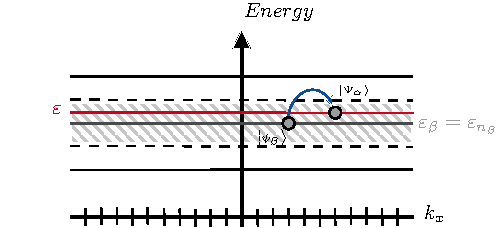
\includegraphics[scale=1.0]{figures/fig2.pdf}
  \caption{Scattering from $\ket{\psi_{\beta}(t,t')}$ to constant energy state $\ket{\Psi_{\alpha}(t,t')}$ due to scattering potential created by impurities.}
  \label{fig:2}
\end{figure}

\noindent
Here we need to undestand a state of this considering system only be represented by two independent quantum numbers which are $n$ energy eigen
states and $k_x = p_x/\hbar$ qunatized momentum in $x$ direction values. Lets calculate the scattering amplitutde of the above mentioned scattering scenario using the equation derived in \eqref{4.18}.
\begin{equation} \label{4.21}
  \begin{aligned}
    a_{\alpha\beta}(\mb{k'},\mb{k},t,t') & =
    -
    \frac{i}{\hbar}
    \int_{0}^t dt_1 \;
    \bra{\psi_{\beta,\mb{k'}}(t_1,t')}
    V(\mb{r}) \ket{\psi_{\alpha,\mb{k}}(t_1,t')} \\
    & =
    -
    \frac{i}{\hbar}
    \int_{0}^t dt_1 \;
    e^{\frac{i}{\hbar}\qty(\varepsilon_{\beta} - \varepsilon)t_1}
    \bra{\phi_{\beta,\mb{k'}}(t')}
    V(\mb{r}) \ket{\phi_{\alpha,\mb{k}}(t')}
  \end{aligned}
\end{equation}
Next assuimg this scenario for long time $t \rightarrow \infty$ we can turn this integral into a delta distrubution as follows
\begin{equation} \label{4.22}
  \begin{aligned}
    a_{\alpha\beta}(\mb{k'},\mb{k},t,t') & =
    -
    \frac{i}{\hbar}
    \lim_{t \rightarrow \infty}\qty[
      \int_{-t/2}^{t/2} dt_1 \;
      e^{\frac{i}{\hbar}\qty(\varepsilon_{\beta} - \varepsilon)t_1}
      \bra{\phi_{\beta,\mb{k'}}(t')}
      V(\mb{r}) \ket{\phi_{\alpha,\mb{k}}(t')}
    ] \\
    & =
    -2\pi i \delta(\varepsilon_{\beta} - \varepsilon)
    \bra{\phi_{\beta,\mb{k'}}(t')}
    V(\mb{r}) \ket{\phi_{\alpha,\mb{k}}(t')}
  \end{aligned}
\end{equation}

\noindent
Now lets consider about the inner product of the above derivation. Using completeness properties we can write that as follows
\begin{equation} \label{4.23}
  \begin{aligned}
    Q & \equiv
    \bra{\phi_{\beta,\mb{k'}}(t')}
    V(\mb{r}) \ket{\phi_{\alpha,\mb{k}}(t')} \\
    & =
    \sum_{\mb{k}}\sum_{\mb{k'}}
    \braket{\phi_{\beta,\mb{k'}}(t')}{\mb{k'}}
    \mel{\mb{k'}}{V(\mb{r})}{\mb{k}}
    \braket{\mb{k}}{\phi_{\alpha,\mb{k}}(t')}
  \end{aligned}
\end{equation}
and seperating $x$ and $y$ directional momentums we can modify this as follows (Assuming $L_y \rightarrow \infty$)
\begin{equation} \label{4.24}
  \begin{aligned}
    Q & \equiv
    \bra{\phi_{\beta,\mb{k'}}(t')}
    V(\mb{r}) \ket{\phi_{\alpha,\mb{k}}(t')} \\
    & =
    \frac{1}{L_y}
    \sum_{k_x}\sum_{{k'}_x}
    \int_{-\infty}^{\infty} \int_{-\infty}^{\infty} dk_y d{k'}_y \;
    \phi_{\beta}(\mb{k'},t')
    \mel{\mb{k'}}{V(\mb{r})}{\mb{k}}
    \phi_{\alpha}(\mb{k},t').
  \end{aligned}
\end{equation}
For a random white scattering potential we can represent the inner product of scattering potential with momentum as a constant value as
\begin{equation} \label{4.25}
  V_{\mb{k'},\mb{k}} \equiv \mel{\mb{k'}}{V(\mb{r})}{\mb{k}}.
\end{equation}
Therefore, using the Eq. \eqref{3.36} the Eq. \eqref{4.24} leads to (we can change varable $t' \rightarrow t$)
\begin{equation} \label{4.26}
  \begin{aligned}
    Q & =
    \sum_{k_x}\sum_{{k'}_x}
    \frac{V_{\mb{k'},\mb{k}}}{L_y}
    \int_{-\infty}^{\infty} \int_{-\infty}^{\infty} dk_y d{k'}_y \; \\
    & \times
    \frac{-i^{n_{\beta}}\sqrt{2\pi}}{\sqrt{L_x}}
    \delta\qty({k'}_x -\frac{p_{x_{\beta}}}{\hbar})
    \exp(
      -ib\sin(2\omega t)
    )
    \exp(
      i{k'}_y  \qty[d\sin(\omega t) + {y'}_0]
    )
    \tilde{\chi}_{n_{\beta}}\qty({k'}_y -g\cos(\omega t))
    \\
    & \times
    \frac{i^{n_{\alpha}}\sqrt{2\pi}}{\sqrt{L_x}}
    \delta\qty(k_x -\frac{p_{x_{\alpha}}}{\hbar})
    \exp(
      ib\sin(2\omega t)
    )
    \exp(
      -ik_y  \qty[d\sin(\omega t) + y_0]
    )
    \tilde{\chi}_{n_{\alpha}}\qty(k_y -g\cos(\omega t))
  \end{aligned}
\end{equation}
and this can re-write as
\begin{equation} \label{4.27}
  \begin{aligned}
    Q =
    \sum_{k_x}\sum_{{k'}_x}
    \frac{-2\pi V_{\mb{k'},\mb{k}} i^{n_{\alpha} + n_{\beta}}}{L_x L_y} &
    \delta\qty({k'}_x -\frac{p_{x_{\beta}}}{\hbar})
    \delta\qty(k_x -\frac{p_{x_{\alpha}}}{\hbar})
    I I'
  \end{aligned}
\end{equation}
where
\begin{equation} \label{4.28}
  \begin{aligned}
    I \equiv
    \int_{-\infty}^{\infty} dk_y \;
    \tilde{\chi}_{n_{\alpha}}\qty(k_y -g\cos(\omega t))
    \exp(
      -ik_y  \qty[d\sin(\omega t) + y_0]
    )
  \end{aligned}
\end{equation}
\begin{equation} \label{4.29}
  \begin{aligned}
    I' \equiv
    \int_{-\infty}^{\infty} d{k'}_y \;
    \tilde{\chi}_{n_{\beta}}\qty({k'}_y -g\cos(\omega t))
    \exp(
      i{k'}_y  \qty[d\sin(\omega t) + {y'}_0]
    )
  \end{aligned}
\end{equation}

\noindent
Lets consider about first integral and we can calculate it as using the following subtitution. Let
\begin{equation} \label{4.30}
  {k}_y -g\cos(\omega t) = \bar{k}_y \longrightarrow d{k}_y = d\bar{k}_y
\end{equation}
and this leads to
\begin{equation} \label{4.31}
    I \equiv
    \int_{-\infty}^{\infty} d\bar{k}_y \;
    \tilde{\chi}_{n_{\alpha}}\qty(\bar{k}_y)
    \exp(
      -i\qty(\bar{k}_y + g\cos(\omega t)) \qty(d\sin(\omega t) + y_0)
    )
\end{equation}
and
\begin{equation} \label{4.32}
    I \equiv
    \exp(g\cos(\omega t)\qty[d\sin(\omega t) + y_0])
    \int_{-\infty}^{\infty} d\bar{k}_y \;
    \tilde{\chi}_{n_{\alpha}}\qty(\bar{k}_y)
    \exp(
      -i\bar{k}_y\qty(d\sin(\omega t) + y_0)
    ).
\end{equation}
Using Fourier transform of Gauss-Hermite functions we can write this as
\begin{equation} \label{4.33}
    I \equiv
    \sqrt{2\pi}
    e^{g\cos(\omega t)\qty[d\sin(\omega t) + y_0]}
    \tilde{\chi}_{n_{\alpha}}\qty(d\sin(\omega t) + y_0)
\end{equation}
Considering second integral with following subtitution and let
\begin{equation} \label{4.34}
  {k'}_y - g\cos(\omega t) = \bar{k'}_y \longrightarrow d{k'}_y = d\bar{k'}_y
\end{equation}
and this leads to
\begin{equation} \label{4.35}
    I' \equiv
    \int_{-\infty}^{\infty} d\bar{k'}_y \;
    \tilde{\chi}_{n_{\beta}}\qty(\bar{k'}_y)
    \exp(
      -i\qty(\bar{k'}_y + g\cos(\omega t)) \qty[-d\sin(\omega t) - {y'}_0]
    )
\end{equation}
and
\begin{equation} \label{4.36}
    I' \equiv
    \exp(-g\cos(\omega t)\qty[d\sin(\omega t) + {y'}_0])
    \int_{-\infty}^{\infty} d\bar{k'}_y \;
    \tilde{\chi}_{n_{\beta}}\qty(\bar{k'}_y)
    \exp(
      -i\bar{k'}_y\qty(d\sin(\omega t) + {y'}_0)
    ).
\end{equation}
Sama as above using Fourier transform of Gauss-Hermite functions we can write this as
\begin{equation} \label{4.37}
    I' \equiv
    \sqrt{2\pi}
    e^{-g\cos(\omega t)\qty[d\sin(\omega t) + {y'}_0]}
    \tilde{\chi}_{n_{\beta}}\qty(-d\sin(\omega t) - {y'}_0)
\end{equation}
Therefore the Eq. \eqref{4.27} becomes
\begin{equation} \label{4.38}
  \begin{aligned}
    Q =
    \sum_{k_x}\sum_{{k'}_x}
    \frac{-4\pi^2 V_{\mb{k'},\mb{k}} i^{n_{\alpha} + n_{\beta}}}{L_x L_y} &
    \delta\qty({k'}_x -\frac{p_{x_{\beta}}}{\hbar})
    \delta\qty(k_x -\frac{p_{x_{\alpha}}}{\hbar})
    e^{g\cos(\omega t)\qty[y_0 - {y'}_0]}\\
    & \times
    \tilde{\chi}_{n_{\alpha}}\qty(d\sin(\omega t) + y_0)
    \tilde{\chi}_{n_{\beta}}\qty(-d\sin(\omega t) - {y'}_0)
  \end{aligned}
\end{equation}



















xxx
